\chapter[Metodologia]{Metodologia}

Neste trabalho foi e será seguido um modelo de pesquisa teórico, aplicado e experimental. Este trabalho é embasado em profunda pesquisa bibliográfica em cima dos temas definidos, que já foram bem abordados por diversos autores anteriormente. Com isso, já há uma metodologia a ser seguida (processo orientado a \textit{hot-spots}) e pesquisas e/ou simuladores nas áreas abordadas (como o MRIT de \cite{Guzman2008} ou as teses de \cite{Souza2008}, \cite{Thomsen2010} e \cite{Strandberg2004}), servindo de guia para implementação e modelo de comparação para os testes realizados.

O tipo de pesquisa (em relação aos objetivos) foi majoriatariamente exploratório, buscando conhecer e compreender a fundo o tema. Foi gasto grande tempo com levantamento bibliográfico, estudando teses e artigos na área e analisando o que se encaixava no tema. Já o tipo de pesquisa para a abordagem (implementação) é híbrida, sendo quantitativa em relação as medidas de desempenho, coesão, acoplamento e qualidade dos resultados apresentado pelos algorítmos (os resultados podem ser comparados com outros estudos e medidos por testes) e qualitaiva quanto as métricas subjetivas como legibilidade do código.

\section{Processo de produção}

Com isso, a metodologia abordada neste trabalho envolve pesquisa sistemática sobre o tema, afim de levantar materiais de estudo ligados ao tema e deles tirar o modo de desenvolver o \textit{framework} e seus algoritmos, além de buscar métricas para comparar o funcionamento do sistema. Com base nestes estudos, será feito então uma prova de conceito, desenvolvendo a arquitetura do sistema e implementado um dos algoritmos para validar a proposta levantada. Após os experimentos a proposta será refinada de acordo com os resultados obtidos.

A partir deste refinamento será dado início a produção do \textit{framework} por completo seguindo o processo orientado a \textit{hot-spot} apresentado por \cite{Fayad1999} em combinação com a metodologia de desenvolvimento Scrum. A abordagem será top-down, focando em cada iteração (ou \textit{sprint}) em uma funcionalidade e no módulo e classes correspondentes a mesma. 

A cada \textit{sprint} espera-se concluir uma tarefa que agregue valor ao produto, podendo ser essa tarefa um algorítmo, um módulo de estrutura de dados (como o Graph ou Map), uma interface e as interações de um componente completa e testada ou um teste da implementação no robô em ambiente controlado. Todo início de ciclo será escolhido uma tarefa a ser atacada, revisada e refinada sua análise, levantado \textit{hot-spots} e desenvolvida e revista sua comunicação com os demais módulos. Será dedicado um tempo para a reavaliação dos \textit{hot-spots} já desenvolvidos também e validação do produto entregue.

\section{Atividades e fluxo de atividades}

Quase todas as atividades foram detalhadas na figura 15. As inserções foram baseadas no processo do Scrum e nas atividades já relizadas ao longo deste trabalho. O diagrama de atividades completo é apresentado na figura 29.

\begin{figure}[h]
	\centering
	\label{fig29}
		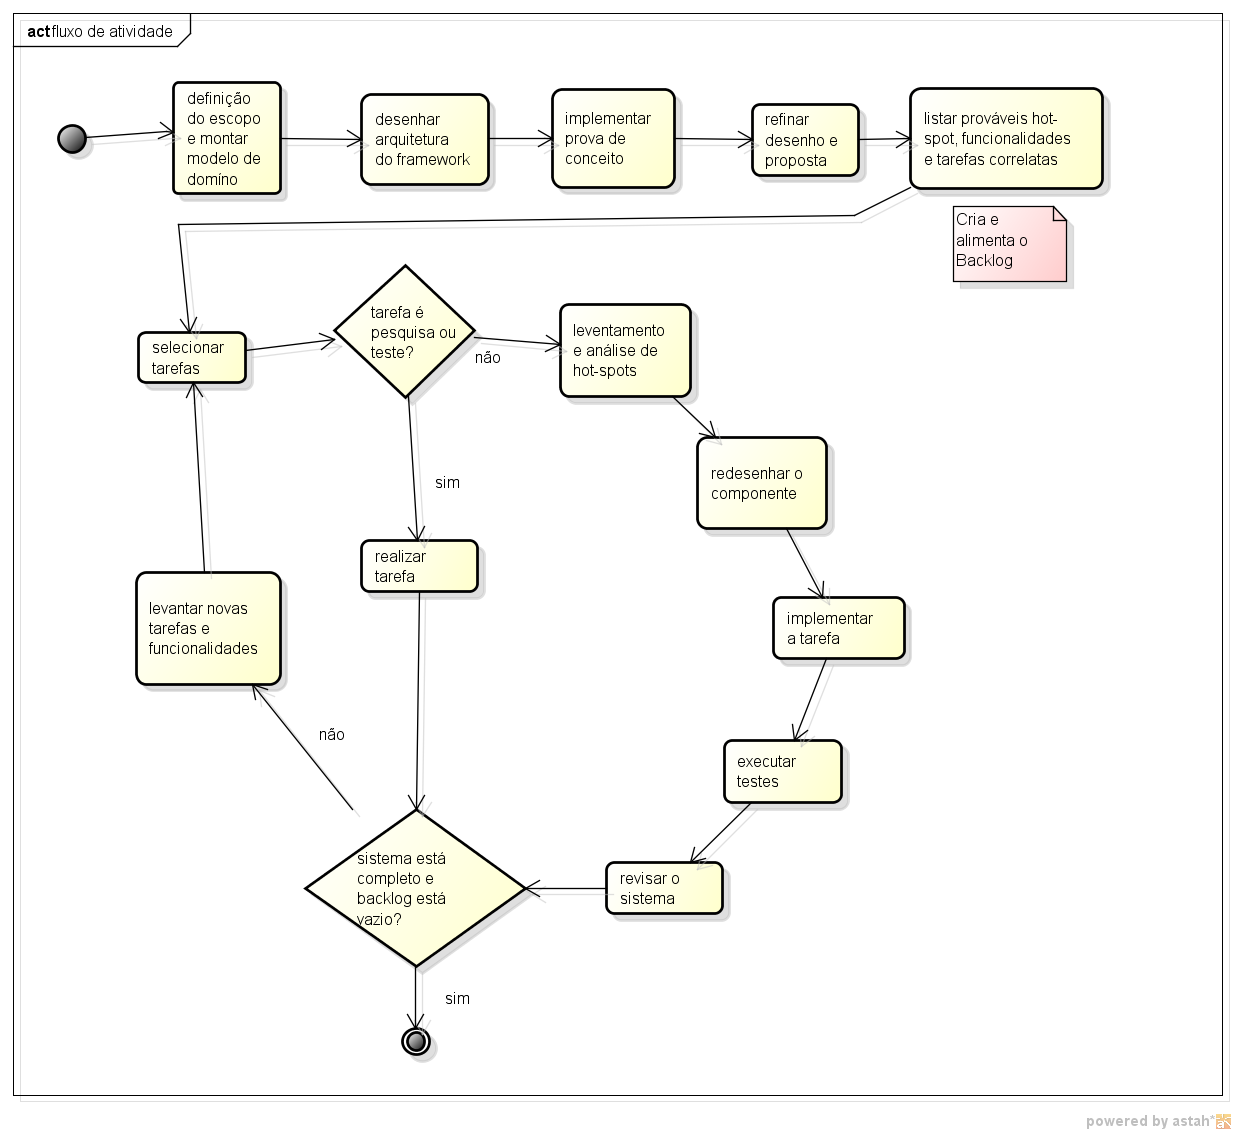
\includegraphics[keepaspectratio=true,scale=0.4]{figuras/fluxoatvd.png}
	\caption{fluxo de atividades propostas}
\end{figure}

As atividades iniciais compõem a definição do tema, estudo do mesmo e execução da prova de conceito. Após seu refiniamento é criado o \textit{backlog} do sistema e alimenta-o com todas as funcionalidades, \textit{hot-spots}, pesquisas e tarefas correlatas a serem realizadas. A partir de então inicia-se as \textit{sprints}, seleciona as tarefas a serem feitas nesta iteração e, caso seja apenas pesquisa ou teste no robô é executada a tarefa e ao seu fim verificado se há mais tarefas para selecioná-las.

Caso seja trabalho sobre o \textit{framework} é analisado se há algum \textit{hot-spot} nas funcionalidades selecionadas, refinado o desenho do componente trabalhado caso necessário para receber a nova funcionalidade e o novo \textit{hot-spot} (se houver) e implementada a funcionalidade nova. Depois é feito uma revisão de todo o sistema para ver se está evoluindo para o fim esperado e se há alguma falha arquitetural. Por fim é verificado se ainda há trabalho a ser feito e, caso haja, levantado mais tarefas, testes e pesquisas para alcançar seu fim.
